\documentclass[aps,pre,twocolumn,superscriptaddress,floatfix]{revtex4-2}
\usepackage{amsmath,amssymb}
\usepackage{graphicx}
\usepackage{hyperref}

\begin{document}

\title{The Lifecycle Equation:\\
Cognition, Emotion, and Aging as Three-Force Competition\\
on an Impedance Network}

\author{Hsi-Yu Huang}
\email{llc.y.huangll@gmail.com}
\affiliation{Independent Researcher, Taiwan}

\date{\today}

\begin{abstract}
Papers~I--III of this series established that Minimum
Reflection Action on impedance networks generates relay-node
hierarchies (Paper~I), governs vascular topology via
Murray's Law and dual-network organ health (Paper~II),
and that time-integrated impedance
mismatch---\emph{impedance debt} $D_Z = D_{Z,n} + D_{Z,v}$---explains
the thermodynamic origin of sleep and brain evolution (Paper~III).
Here we derive the \emph{Lifecycle Equation},
\begin{equation*}
  \frac{d(\Sigma\Gamma^2)}{dt}
    = \underbrace{-\eta\,\Sigma\Gamma^2}_{\text{learning}}
    + \underbrace{\gamma\,\Gamma_{\mathrm{env}}(t)}_{\text{novelty}}
    + \underbrace{\delta\,D(t)}_{\text{aging}}\,,
\end{equation*}
governing the complete cognitive trajectory from birth to
senescence as a three-force competition on the dual
neural--vascular impedance network.
Learning (MRP descent) reduces mismatch; environmental
novelty injects fresh mismatch; irreversible fatigue damage
(Coffin--Manson mechanics) drifts impedance away from match.
The resulting \emph{bathtub curve} of $\Sigma\Gamma^2$---high at
birth, rapidly falling in infancy, plateauing in adulthood,
and rising again in senescence---reproduces the known
developmental trajectory of cognitive performance without
any fitted function.
Emotion, reward, stress, curiosity, and boredom emerge as
\emph{readouts} of $\Gamma$ dynamics at different time scales:
dopamine encodes $-\Delta\Gamma^2$ (reward = impedance
mismatch reduction), cortisol encodes chronic $\Gamma^2$
elevation (stress = sustained mismatch),
curiosity encodes $\partial\Gamma^2/\partial(\text{novelty})$
(information hunger = impedance gradient),
and boredom encodes $\partial\Gamma^2/\partial t \to 0$
at high $\Gamma^2$ (stagnation without resolution).
Nine computational experiments verify these predictions,
including the Yerkes--Dodson inverted-U curve as an
impedance-matching optimum, chronic stress as Arrhenius-accelerated
fatigue, and the full lifecycle simulation from birth to
senescence with emergent phase transitions.
Atherosclerosis is derived as vascular Coffin--Manson fatigue,
and the dual-network aging cascade
($\Gamma_v\!\uparrow \to \rho\!\downarrow \to \Gamma_n\!\uparrow$)
explains why cardiovascular disease precedes and accelerates
neurodegeneration---unifying the vascular and neural theories
of aging within a single variational principle.
The Equilibrium Equation,
$T_{\mathrm{steady}} = T_{\mathrm{env}} + (\alpha/\beta)\,\Sigma\Gamma^2$,
gives adulthood a physical definition:
the thermal steady state at which the world can no longer
burn you.
\end{abstract}

\maketitle


% ============================================================
%  SECTION 1 — INTRODUCTION
% ============================================================
\section{Introduction}
\label{sec:intro}

Why do children learn so fast?
Why does stress impair memory?
Why does cognitive performance follow a
bathtub curve---high error at birth, rapid improvement
in childhood, a long plateau, and gradual decline in old age?
These questions span developmental psychology~\cite{Kail1991},
stress physiology~\cite{McEwen1998},
and gerontology~\cite{Salthouse2010},
yet no single equation unifies them.

In Paper~I~\cite{PaperI} we showed that the Minimum
Reflection Action $\mathcal{A}[\Gamma] = \int |\Gamma|^2\,dt$
on an impedance-heterogeneous network forces hierarchical
relay-node emergence, with dimensional cut cost $A_{\mathrm{cut}}$
irreducible by any local rule.
Paper~II~\cite{PaperII} extended the framework to vascular
networks, deriving Murray's Law from the same variational
principle and establishing the dual-network organ model.
Paper~III~\cite{PaperIII} extended the framework to the time domain:
the integral of $|\Gamma|^2$ weighted by incident power
defines impedance debt $D_Z$, whose homeostatic discharge
is sleep, whose centralised management is the brain,
and whose material-supply dependence produces morphogenesis.

This fourth paper asks: what happens to $\Sigma\Gamma^2$
over an \emph{entire lifetime}?
The answer is a first-order ODE---the \emph{Lifecycle Equation}
---in which three competing physical forces determine the
complete cognitive trajectory.
Cognition, emotion, reward, stress, curiosity, and boredom
are not separate psychological constructs but different
\emph{readouts} of the same impedance-mismatch dynamics
at different time scales.


% ============================================================
%  SECTION 2 — PHYSICAL FRAMEWORK
% ============================================================
\section{Physical Framework}
\label{sec:framework}

\subsection{Review: impedance mismatch and the MRP}

At every signalling interface in a nervous system,
incident power splits into transmitted and reflected
components according to the reflection coefficient
\begin{equation}
  \Gamma = \frac{Z_{\mathrm{load}} - Z_{\mathrm{source}}}
               {Z_{\mathrm{load}} + Z_{\mathrm{source}}}\,,
  \label{eq:gamma}
\end{equation}
with energy conservation enforcing $\Gamma^2 + T = 1$
at every interface, every instant (Constraint~C1).
The Minimum Reflection Principle (MRP) states that
biological networks evolve to minimise the total action
$\mathcal{A}[\Gamma] = \sum_i \int_0^T \Gamma_i^2(t)\,dt$.
Hebbian plasticity is the gradient descent:
$\Delta Z = -\eta\,\Gamma\,x_{\mathrm{pre}}\,
x_{\mathrm{post}}$ (Constraint~C2).

\subsection{The total mismatch energy: $\Sigma\Gamma^2$}

Define the \emph{total normalised mismatch energy}
as the population-averaged squared reflection coefficient:
\begin{equation}
  \Sigma\Gamma^2(t) \equiv
    \frac{1}{N} \sum_{i=1}^{N} \Gamma_i^2(t)\,,
  \label{eq:sigma-gamma}
\end{equation}
where $N$ is the number of signalling interfaces.
$\Sigma\Gamma^2 = 1$ corresponds to total reflection
(no information transmits); $\Sigma\Gamma^2 = 0$
to perfect matching (all information transmits).
The complement $\Sigma T = 1 - \Sigma\Gamma^2$ is
the system's \emph{cognitive throughput}.


\subsection{Dual-network extension}
\label{sec:dual-lifecycle}

Paper~II~\cite{PaperII} established that organ health depends
on \emph{two} impedance networks:
$H = (1-\Gamma_n^2)(1-\Gamma_v^2)$.
Paper~III~\cite{PaperIII} extended this to impedance debt:
$D_Z = D_{Z,n} + D_{Z,v}$.
The lifecycle equation inherits the same dual structure.

We decompose the total mismatch energy into neural and
vascular components:
\begin{equation}
  \Sigma\Gamma^2 = \Sigma\Gamma_n^2 + w_v\,\Sigma\Gamma_v^2\,,
  \label{eq:sigma-gamma-dual}
\end{equation}
where $w_v = \alpha_{v\to n}$ is the vascular-to-neural
coupling weight from Paper~II
($\alpha_{v\to n} = 0.5$ in the Alice simulator).
The two components evolve on different time scales:
neural $\Gamma_n$ changes on millisecond-to-hour time scales
(synaptic plasticity), while vascular $\Gamma_v$ changes on
day-to-year time scales (vessel-wall remodeling,
angiogenesis).
This time-scale separation means that the neural and vascular
bathtub curves (Sec.~\ref{sec:bathtub}) have different shapes:
the neural curve descends rapidly in infancy, while the
vascular curve follows later and rises earlier in aging
---a prediction we verify in Sec.~\ref{sec:exp1}.


\subsection{Three forces acting on $\Sigma\Gamma^2$}

Three physically distinct mechanisms alter the impedance
landscape and hence $\Sigma\Gamma^2$:

\emph{(i)~Learning (MRP descent).}
Hebbian plasticity (C2) adapts $Z_{\mathrm{load}}$
toward $Z_{\mathrm{source}}$, reducing $\Gamma_i^2$
at every active interface.
The aggregate effect is an exponential relaxation:
\begin{equation}
  \left.\frac{d(\Sigma\Gamma^2)}{dt}\right|_{\mathrm{learn}}
    = -\eta(t)\,\Sigma\Gamma^2\,,
  \label{eq:learning-term}
\end{equation}
where $\eta(t)$ is the effective learning rate,
modulated by sleep quality (consolidation),
attention (gain), and developmental stage
(critical-period enhancement).

\emph{(ii)~Novelty injection.}
Each new stimulus introduces impedance mismatches
at interfaces that have not yet been tuned.
An infant in a novel world experiences $\Gamma_{\mathrm{env}}
\approx 1$ at nearly every channel;
an adult in a familiar environment experiences
$\Gamma_{\mathrm{env}} \approx 0$ at most channels.
The aggregate novelty injection is:
\begin{equation}
  \left.\frac{d(\Sigma\Gamma^2)}{dt}\right|_{\mathrm{novel}}
    = \gamma(t)\,\Gamma_{\mathrm{env}}(t)\,,
  \label{eq:novelty-term}
\end{equation}
where $\gamma(t)$ decreases with cumulative exposure
(habituation) and $\Gamma_{\mathrm{env}}(t)$ encodes
the current environmental novelty intensity.

\emph{(iii)~Aging (Coffin--Manson fatigue).}
Repeated current flow through neural tissue produces
irreversible mechanical strain via the Lorentz
pinch effect~\cite{Coffin1954}:
\begin{equation}
  \varepsilon_{\mathrm{pinch}} = S\,|I|^\alpha\,,
  \label{eq:pinch}
\end{equation}
where $S$ is the pinch sensitivity, $\alpha \approx 2$
the force exponent, and $I$ the current amplitude.
Strains exceeding the yield threshold $\varepsilon_y$
produce permanent (plastic) deformation that drifts
$Z_{\mathrm{load}}$ away from $Z_{\mathrm{source}}$,
increasing $\Gamma^2$.
The cumulative fatigue damage $D(t)$ follows the
Coffin--Manson power law.
Stress accelerates this process via Arrhenius kinetics:
\begin{equation}
  \delta_{\mathrm{eff}}(t) = \delta_0\,
    \exp\!\bigl(E_a\,\sigma_{\mathrm{stress}}(t)\bigr)\,,
  \label{eq:arrhenius-aging}
\end{equation}
where $E_a$ is an effective activation energy and
$\sigma_{\mathrm{stress}}$ the chronic stress level.
The aging term is:
\begin{equation}
  \left.\frac{d(\Sigma\Gamma^2)}{dt}\right|_{\mathrm{age}}
    = \delta_{\mathrm{eff}}(t)\,D(t)\,.
  \label{eq:aging-term}
\end{equation}


\subsection{The Lifecycle Equation}
\label{sec:lifecycle-eq}

Combining the three forces yields the
\emph{Lifecycle Equation}:
\begin{equation}
  \boxed{\;
  \frac{d(\Sigma\Gamma^2)}{dt}
    = -\eta\,\Sigma\Gamma^2
    + \gamma\,\Gamma_{\mathrm{env}}(t)
    + \delta\,D(t)
  \;}
  \label{eq:lifecycle}
\end{equation}
This is a non-autonomous first-order ODE whose
coefficients $\eta(t)$, $\gamma(t)$, $\delta(t)$
are themselves functions of developmental stage,
environmental statistics, and cumulative damage.
No fitted function is required: the bathtub curve
emerges from the relative magnitudes of three
physically motivated terms.


\subsection{The Equilibrium Equation}
\label{sec:equilibrium}

Impedance mismatch dissipates energy as heat.
The thermal balance of neural tissue gives:
\begin{equation}
  C\,\frac{dT}{dt} = \alpha\,\Sigma\Gamma^2\,\bar{P}
    - \beta\,(T - T_{\mathrm{env}})\,,
  \label{eq:thermal}
\end{equation}
where $C$ is heat capacity, $\alpha$ the fraction of
reflected power converted to heat, and $\beta$ the
cooling coefficient (blood flow, radiation, conduction).
At steady state:
\begin{equation}
  T_{\mathrm{steady}} = T_{\mathrm{env}}
    + \frac{\alpha}{\beta}\,\Sigma\Gamma^2\,.
  \label{eq:equilibrium}
\end{equation}
This is the \emph{Equilibrium Equation}:
the neural tissue temperature at which
waste-heat generation equals dissipation.
It gives ``adulthood'' a physical definition---the
thermal steady state reached when
$d(\Sigma\Gamma^2)/dt \approx 0$ and the system
has reached its minimum-action configuration
compatible with the current environment and
accumulated damage.


\subsection{Emotion as $\Gamma$-dynamics readout}
\label{sec:emotion}

Psychological states map to specific features
of the $\Gamma^2$ time series:

\begin{itemize}
  \item \textbf{Reward (dopamine)}:
    $r = -\Delta\Gamma^2 / \Delta t$.
    Impedance mismatch \emph{reduction} releases dopamine.
    Prediction error in reinforcement learning is
    the \emph{rate of impedance matching}.

  \item \textbf{Pain / aversive signal}:
    $p = +\Delta\Gamma^2 / \Delta t$.
    Sudden mismatch \emph{increase} signals tissue damage
    or environmental threat.

  \item \textbf{Stress (cortisol)}:
    $s = \langle\Gamma^2\rangle_{\tau_{\mathrm{slow}}}$,
    time-averaged over a slow (hours--days) window.
    Chronic mismatch elevation, not acute spikes,
    drives HPA axis activation.

  \item \textbf{Curiosity}:
    $c = \partial\Gamma^2 / \partial(\text{novelty})
    \big|_{\Gamma^2 < \Gamma^2_{\mathrm{threat}}}$.
    The impedance gradient with respect to novelty,
    gated by the condition that current mismatch is
    not threatening.
    ``I want to explore because the gradient is steep
    and I am not in danger.''

  \item \textbf{Boredom}:
    $b = \mathbb{1}\!\bigl[
      |d\Gamma^2/dt| < \epsilon
      \;\wedge\;
      \Gamma^2 > \Gamma^2_{\mathrm{target}}
    \bigr]$.
    Stagnation \emph{at non-zero mismatch}:
    the system is stuck but not matched.
    Low derivative + high $\Gamma^2$ = unresolved
    impedance debt with no learning progress.

  \item \textbf{Flow state}:
    The condition $\Gamma^2 \approx \Gamma^2_{\mathrm{optimal}}$
    where $d\Gamma^2/dt < 0$ (still improving)
    and $|\Gamma^2|$ matches the Yerkes--Dodson optimum---
    challenge equals skill.
\end{itemize}

Each ``emotion'' is a temporal filter on the same
underlying physical variable $\Gamma^2$, differing
only in time scale (milliseconds for reward prediction
error, hours for stress, years for aging)
and in the derivative order (level, rate, acceleration,
integral).


% ============================================================
%  SECTION 3 — THE BATHTUB CURVE
% ============================================================
\section{The Bathtub Curve of Cognition}
\label{sec:bathtub}

\subsection{Qualitative trajectory}

The Lifecycle Equation~\eqref{eq:lifecycle} predicts
six developmental phases governed by the relative
magnitudes of the three terms:

\begin{enumerate}
  \item \textbf{Birth} ($t = 0$):
    $\Sigma\Gamma^2 \approx 0.8$--$1.0$.
    Random initialisation; nearly all interfaces mismatched.
    Novelty $\gg$ Learning $\gg$ Aging.

  \item \textbf{Infancy} ($t < t_1$):
    Learning term dominates.
    $\eta$ is maximal (critical period);
    $\Sigma\Gamma^2$ drops rapidly.
    Neural pruning eliminates chronically mismatched
    synapses---the impedance-mismatch interpretation of
    apoptosis~\cite{Huttenlocher1979}.

  \item \textbf{Childhood} ($t_1 < t < t_2$):
    Learning $\approx$ Novelty.
    Intense consolidation; $\Sigma\Gamma^2$ decreases
    steadily but more slowly than in infancy.
    REM sleep fraction is high because the topological
    complexity $N$ of the $Z$-map is still growing
    (Paper~III, Eq.~(9)).

  \item \textbf{Adulthood} ($t_2 < t < t_3$):
    $d(\Sigma\Gamma^2)/dt \approx 0$.
    Learning $\approx$ Novelty + Aging.
    The system has reached its minimum-action configuration.
    The Equilibrium Equation~\eqref{eq:equilibrium} gives
    the steady-state temperature:
    ``the point at which the world can no longer burn you.''

  \item \textbf{Decline} ($t_3 < t < t_4$):
    Aging $>$ Learning.
    Cumulative fatigue damage $D(t)$ causes net mismatch
    increase despite continued learning.
    $\Sigma\Gamma^2$ rises slowly.

  \item \textbf{Senescence} ($t > t_4$):
    Aging $\gg$ Learning.
    Cascading failure: rising $\Gamma^2$ increases
    current flow through remaining channels (compensation),
    which accelerates fatigue in a positive feedback loop.
    System failure occurs when $\Sigma\Gamma^2$ exceeds
    a viability threshold.
\end{enumerate}

\subsection{The bathtub as reliability curve}

The $\Sigma\Gamma^2$ trajectory is formally identical
to the \emph{bathtub curve} of engineering reliability
theory~\cite{Klutke2003}:
early ``infant mortality'' (burn-in failures),
a long ``useful life'' (random failures at constant
low rate), and ``wear-out'' (increasing failure rate).
This is not an analogy but a \emph{derivation}:
both phenomena arise from the same physics---
impedance mismatch in a transmission network subject
to random perturbations and irreversible fatigue.


% ============================================================
%  SECTION 4 — EMOTION AS IMPEDANCE DYNAMICS
% ============================================================
\section{Emotion as Impedance Dynamics}
\label{sec:emotion-detail}

\subsection{Dopamine: the $-\Delta\Gamma^2$ signal}

The reward prediction error (RPE) of reinforcement
learning~\cite{Schultz1997} is conventionally written
$\delta = r + \gamma V(s') - V(s)$.
In the impedance framework, $V(s)$ is the expected
$\Sigma\Gamma^2$ at state $s$, and the RPE becomes:
\begin{equation}
  \delta_{\mathrm{RPE}} = -\bigl(\Sigma\Gamma^2_{t+1}
    - \mathbb{E}[\Sigma\Gamma^2_{t+1}]\bigr)\,.
  \label{eq:rpe}
\end{equation}
Dopamine fires when mismatch decreases \emph{more than
expected}---the physical interpretation is that
the impedance network matched faster than predicted.
This explains why novelty generates dopamine:
a novel stimulus with $\Gamma_{\mathrm{env}} \gg 0$
that is quickly matched ($\Delta\Gamma^2 \ll 0$)
produces a large RPE.

\subsection{Cortisol: the slow $\Gamma^2$ integrator}

Cortisol release correlates with sustained HPA axis
activation~\cite{McEwen1998}.
In the impedance framework, stress is the
\emph{time-averaged} mismatch energy:
\begin{equation}
  \sigma_{\mathrm{stress}}(t) =
    \frac{1}{\tau_s} \int_{t-\tau_s}^{t}
    \Sigma\Gamma^2(t')\,dt'\,,
  \label{eq:cortisol}
\end{equation}
where $\tau_s \sim$ hours--days is the HPA integration
time constant.
Acute stress (exam, confrontation) raises
$\Sigma\Gamma^2$ transiently; the cortisol response
activates only if the elevation persists beyond
$\tau_s$---explaining why brief challenges are
stimulating but prolonged ones are harmful.

\subsection{The Yerkes--Dodson curve as impedance optimum}
\label{sec:yerkes-dodson}

The Yerkes--Dodson inverted-U relationship between
arousal and performance~\cite{YerkesDodson1908}
emerges naturally from the Lifecycle Equation.
Performance (cognitive throughput) is
$\Sigma T = 1 - \Sigma\Gamma^2$.
Arousal increases the learning rate $\eta$
(via noradrenergic modulation) but also increases
the novelty injection rate $\gamma$ (more inputs
processed per unit time).
At low arousal, $\eta$ is small and learning is slow.
At high arousal, $\gamma$ overwhelms $\eta$ and
net mismatch increases.
The optimum occurs at the arousal level where
$d(\Sigma\Gamma^2)/dt$ is most negative:
\begin{equation}
  \eta^*\,\Sigma\Gamma^2
    = \gamma^*\,\Gamma_{\mathrm{env}}
  \quad\Longrightarrow\quad
  \text{arousal}^* = \frac{\eta^*}{\gamma^*}\,
    \frac{\Sigma\Gamma^2}{\Gamma_{\mathrm{env}}}\,.
  \label{eq:yerkes-dodson}
\end{equation}
This predicts that optimal arousal depends on task
difficulty ($\Gamma_{\mathrm{env}}$) and current skill
level ($\Sigma\Gamma^2$)---precisely the
Yerkes--Dodson observation.


\subsection{Curiosity and boredom as impedance gradients}
\label{sec:curiosity-boredom}

Curiosity is the \emph{impedance gradient}:
the expected rate of mismatch reduction per unit
of exploration effort.
Formally:
\begin{equation}
  \mathcal{C} = -\frac{\partial(\Sigma\Gamma^2)}
    {\partial(\text{exploration})}
  \bigg|_{\Gamma^2 < \Gamma^2_{\mathrm{threat}}}\,.
  \label{eq:curiosity}
\end{equation}
When the gradient is steep (novel but non-threatening
stimuli), curiosity is high.
When the gradient is flat (familiar environment or
overwhelmingly complex stimuli), curiosity diminishes.

Boredom arises when:
\begin{equation}
  \left|\frac{d(\Sigma\Gamma^2)}{dt}\right| < \epsilon
  \quad\text{and}\quad
  \Sigma\Gamma^2 > \Gamma^2_{\mathrm{target}}\,.
  \label{eq:boredom}
\end{equation}
The system is stuck at non-zero mismatch with no
learning progress.
This produces an intrinsic drive to seek new stimuli---
not as a ``psychological need'' but as a
\emph{thermodynamic imperative}: the system must increase
$\Gamma_{\mathrm{env}}$ to find new gradients along
which $\mathcal{A}[\Gamma]$ can be further reduced.


\subsection{Metacognition as second-order $\Gamma$ monitoring}
\label{sec:metacognition}

Self-awareness requires the system to monitor its own
impedance dynamics.
Define the \emph{thinking impedance}:
\begin{equation}
  \Gamma_{\mathrm{think}} =
    \frac{\sum_i w_i\,\Gamma_i}{\sum_i w_i}\,,
  \label{eq:gamma-think}
\end{equation}
a weighted average of impedance mismatches across
cognitive channels.
Two distinct processing modes emerge:
\begin{itemize}
  \item \textbf{System~1 (intuition)}:
    $\Gamma_{\mathrm{think}} < \Gamma_{\mathrm{S2}}$.
    Low mismatch; fast, automatic processing.
  \item \textbf{System~2 (deliberation)}:
    $\Gamma_{\mathrm{think}} > \Gamma_{\mathrm{S2}}$.
    High mismatch triggers slow, effortful processing
    with increased metabolic cost~\cite{Kahneman2011}.
\end{itemize}
The switching threshold $\Gamma_{\mathrm{S2}}$ provides
a physics-based mechanism for dual-process theory.
Confidence estimation follows as
$\mathrm{Conf} = 1/(1 + \sigma^2 + \Gamma_{\mathrm{think}})$,
where $\sigma^2$ is prediction variance---matching
the experimental finding that confidence correlates
with both fluency (low $\Gamma$) and low uncertainty
(low $\sigma$)~\cite{Alter2009}.


% ============================================================
%  SECTION 5 — STRESS AND AGING
% ============================================================
\section{Stress, Fatigue, and the Physics of Aging}
\label{sec:aging}

\subsection{Coffin--Manson fatigue in neural tissue}

Every action potential generates a Lorentz force
on conductors carrying current in the tissue's
self-generated magnetic field.
The resulting mechanical strain accumulates according
to the Coffin--Manson law~\cite{Coffin1954}:
\begin{equation}
  N_f = C\,(\Delta\varepsilon_p)^{-\beta}\,,
  \label{eq:coffin-manson}
\end{equation}
where $N_f$ is cycles to failure, $\Delta\varepsilon_p$
the plastic strain range, and $C$, $\beta$ are
material constants.
In biological tissue, ``failure'' corresponds to
irreversible impedance drift: the axon's characteristic
impedance permanently shifts from its target value.


\subsection{Vascular Coffin--Manson: atherosclerosis as fatigue}
\label{sec:vascular-aging}

The same Coffin--Manson physics applies to the vascular
impedance network of Paper~II~\cite{PaperII}.
Every cardiac cycle imposes pulsatile shear stress on the
endothelial lining and circumferential strain on the
vessel wall.
With $\sim$100\,000 beats per day and $\sim$3 billion beats
in a lifetime, vascular tissue undergoes the most extreme
fatigue loading of any organ system.

The vascular plastic strain per cycle is
\begin{equation}
  \varepsilon_{v,\mathrm{plastic}} = S_v\,
    |\Delta P|^{\alpha_v}\,,
  \label{eq:vascular-pinch}
\end{equation}
where $S_v$ is the vessel-wall sensitivity and
$\Delta P$ the pulse pressure.
Cumulative vascular damage $D_v(t)$ drifts
$Z_v$ away from Murray's-Law optimum (Paper~II,
Eq.~(9)), increasing $\Gamma_v^2$.
Atherosclerotic plaque is the macroscopic manifestation
of this impedance drift: intimal thickening narrows
the lumen, increasing $Z_v = 8\mu L/(\pi r^4)$
according to the $r^{-4}$ Poiseuille law,
so that a 50\% stenosis raises $Z_v$ by $16\times$
and drives $\Gamma_v \to 1$.

The vascular aging term in the lifecycle equation is:
\begin{equation}
  \left.\frac{d(\Sigma\Gamma_v^2)}{dt}\right|_{\mathrm{age}}
    = \delta_v\,D_v(t)\,,
  \label{eq:vascular-aging-term}
\end{equation}
paralleling the neural term (Eq.~\eqref{eq:aging-term}),
with $\delta_v > \delta_n$ because vascular tissue
endures far more fatigue cycles per unit time.


\subsection{The vascular--neural aging cascade}
\label{sec:aging-cascade}

The dual-network architecture creates an asymmetric aging
cascade (Paper~II, Eq.~(12)):
\begin{equation}
  D_v\!\uparrow \;\to\;
    \Gamma_v\!\uparrow \;\to\;
    \rho\!\downarrow \;\to\;
    \eta_{n,\mathrm{eff}}\!\downarrow \;\to\;
    \Gamma_n\!\uparrow\,.
  \label{eq:aging-cascade}
\end{equation}
Vascular aging ($D_v$) reduces material supply ($\rho$),
which slows neural Hebbian adaptation ($\eta_{n,\mathrm{eff}}
= \eta_n\,f(\rho)$), causing neural mismatch to rise
even before neural-intrinsic fatigue would predict.
This explains three well-established clinical observations:
\begin{itemize}
  \item \emph{Cardiovascular disease precedes dementia} by
    10--20 years (vascular bathtub rises before neural).
  \item \emph{Blood-pressure control in midlife} reduces late-life
    dementia risk (SPRINT-MIND~\cite{sprint2019}): reducing
    $\Gamma_v$ preserves $\rho$ and hence $\eta_{n,\mathrm{eff}}$.
  \item \emph{Metabolic syndrome} combines both high $\Sigma\Gamma_v^2$
    (hypertension, dyslipidemia) and rising $\Sigma\Gamma_n^2$
    (cognitive decline)---dual failure in the lifecycle framework.
\end{itemize}

\subsection{Elastic vs plastic deformation}

Each current pulse produces total strain
$\varepsilon = \varepsilon_{\mathrm{elastic}}
+ \varepsilon_{\mathrm{plastic}}$.
The elastic component is fully recoverable
(by sleep: Paper~III, impedance debt discharge).
The plastic component is \emph{irreversible}---it
accumulates over a lifetime and cannot be repaired
by any amount of sleep.
This decomposition maps directly onto the
observation that sleep restores daily cognitive
performance but cannot prevent long-term
aging~\cite{Walker2017}.

\subsection{Stress as Arrhenius acceleration}

Chronic stress increases the effective ``temperature''
of fatigue kinetics via the Arrhenius factor
(Eq.~\eqref{eq:arrhenius-aging}).
At stress level $\sigma = 0.5$, the aging rate
accelerates by a factor of $\sim 2.1\times$;
at $\sigma = 1.0$, by $\sim 4.5\times$.
This provides a quantitative mechanism for the
well-established observation that chronic
psychosocial stress accelerates biological
aging~\cite{Epel2004}.

Crucially, the Arrhenius acceleration is
\emph{multiplicative} with cumulative damage:
the aging term is $\delta_{\mathrm{eff}} \cdot D(t)$,
not $\delta_{\mathrm{eff}}$ alone.
A young organism under chronic stress
($\delta_{\mathrm{eff}}$ high, $D(t)$ low)
shows modest effects;
an old organism under the same stress
($\delta_{\mathrm{eff}}$ high, $D(t)$ high)
shows catastrophic decline.
This explains the clinical observation that
elderly individuals are far more vulnerable
to stress-induced cognitive decline than
young adults~\cite{Lupien2009}.


\subsection{Death as positive-feedback collapse}

When $\Sigma\Gamma^2$ rises above a critical threshold,
a destructive positive-feedback loop activates:
high $\Gamma^2$ forces compensatory current increases
through remaining functional channels,
which increases Lorentz pinch strain,
which accelerates fatigue,
which further increases $\Gamma^2$.
In the dual-network framework, this collapse is amplified:
vascular $\Gamma_v\!\uparrow$ starves neural tissue of
material ($\rho\!\downarrow$), accelerating neural $\Gamma_n\!\uparrow$,
which impairs autonomic vascular regulation,
further raising $\Gamma_v$---the positive-feedback cascade
of Paper~II~\cite{PaperII} and Eq.~\eqref{eq:aging-cascade}.
The system enters a supercritical regime where
$d(\Sigma\Gamma^2)/dt$ itself accelerates:
\begin{equation}
  \frac{d^2(\Sigma\Gamma^2)}{dt^2} > 0
  \quad\Longrightarrow\quad
  \text{runaway failure}\,.
  \label{eq:runaway}
\end{equation}
This is the impedance-physics definition of
\emph{senescence}: the point beyond which
the system's repair mechanisms cannot keep pace
with damage accumulation, and cascading failure
becomes inevitable.


% ============================================================
%  SECTION 6 — SLEEP IN THE LIFECYCLE CONTEXT
% ============================================================
\section{Sleep Across the Lifecycle}
\label{sec:sleep-lifecycle}

Paper~III established that sleep discharges impedance
debt $D_Z$.
The Lifecycle Equation adds developmental context:
\emph{how much} sleep is needed depends on the balance
of the three forces.

\subsection{Infant sleep: clearing the initialisation debt}

At birth, $\Sigma\Gamma^2 \approx 0.8$:
nearly all interfaces are mismatched.
The learning rate $\eta$ is maximal
(critical-period plasticity),
but the sheer magnitude of $\Sigma\Gamma^2$
means that daily impedance debt $D_Z$ is enormous.
Infants therefore require 14--17 hours of sleep per day
---not because they are ``immature'' but because the
impedance debt accumulated per waking hour is
proportionally much larger.

REM sleep fraction is maximal ($\sim$50\% of total sleep
in neonates vs $\sim$25\% in adults) because the
topological complexity $N$ of the developing $Z$-map
is rapidly increasing as new connections form
(Paper~III, Eq.~(9): $T_{\mathrm{REM}} \propto N$).

\subsection{Adult sleep: maintenance mode}

In adulthood, $\Sigma\Gamma^2$ is near its minimum.
Daily impedance debt is proportional to
$\langle\Gamma^2\rangle \cdot P_{\mathrm{in}} \cdot
T_{\mathrm{wake}}$ (Paper~III, Eq.~(4)),
but $\langle\Gamma^2\rangle$ is now small.
The 7--9 hours typical of adult sleep suffice to
discharge this modest daily accumulation.

\subsection{Elderly sleep: diminished returns}

In senescence, sleep architecture degrades:
reduced slow-wave sleep, more frequent awakenings,
and decreased sleep efficiency~\cite{Ohayon2004}.
In the lifecycle framework, this occurs because
the irreversible (plastic) component of impedance
drift is \emph{not dischargeable by sleep}.
Sleep can still repair the elastic (daily) component,
but the growing plastic baseline means that even
perfect sleep cannot return $\Sigma\Gamma^2$ to
its youthful minimum.

The dual-network framework adds a second mechanism:
rising vascular $\Gamma_v$ (atherosclerosis,
Sec.~\ref{sec:vascular-aging}) reduces material supply
$\rho = (1-\Gamma_v^2)\,Q_0$, which slows neural
debt discharge ($\eta_{n,\mathrm{eff}} = \eta_n\,f(\rho)$,
Paper~III).
Elderly sleep is therefore doubly impaired:
the plastic neural baseline rises \emph{and}
the vascular supply that enables sleep-mediated repair
simultaneously declines---a prediction consistent with
the observation that sleep quality declines
correlate with both cognitive aging \emph{and}
cardiovascular burden~\cite{Mander2017}.


% ============================================================
%  SECTION 7 — COMPUTATIONAL VERIFICATION
% ============================================================
\section{Computational Verification}
\label{sec:computation}

All simulations use the Alice Gamma-Net framework
with physics constraints C1--C3 enforced at every
time step.
Source code is available in the project repository.

\subsection{Experiment~1: Bathtub curve emergence}
\label{sec:exp1}

We integrate the Lifecycle Equation~\eqref{eq:lifecycle}
for $T = 5000$ ticks (representing a full lifespan)
with parameters:
$\eta_0 = 0.04$ (doubled during critical period,
ticks 0--500),
$\gamma_0 = 0.20$ (decaying with habituation),
$\delta_0 = 10^{-4}$ (activating at tick 1000),
initial $\Sigma\Gamma^2 = 0.8$.

\emph{Verification criteria}:
(a)~$\Sigma\Gamma^2$ drops from $0.8$ to
$< 0.2$ by tick 600 (childhood learning);
(b)~plateau at $\Sigma\Gamma^2 \approx 0.1$--$0.2$
for ticks 1000--3000 (adulthood);
(c)~rise above $0.3$ after tick 4000 (senescence);
(d)~all six developmental phases detected in sequence
(Fig.~\ref{fig:bathtub}).

\begin{figure*}[t]
  \centering
  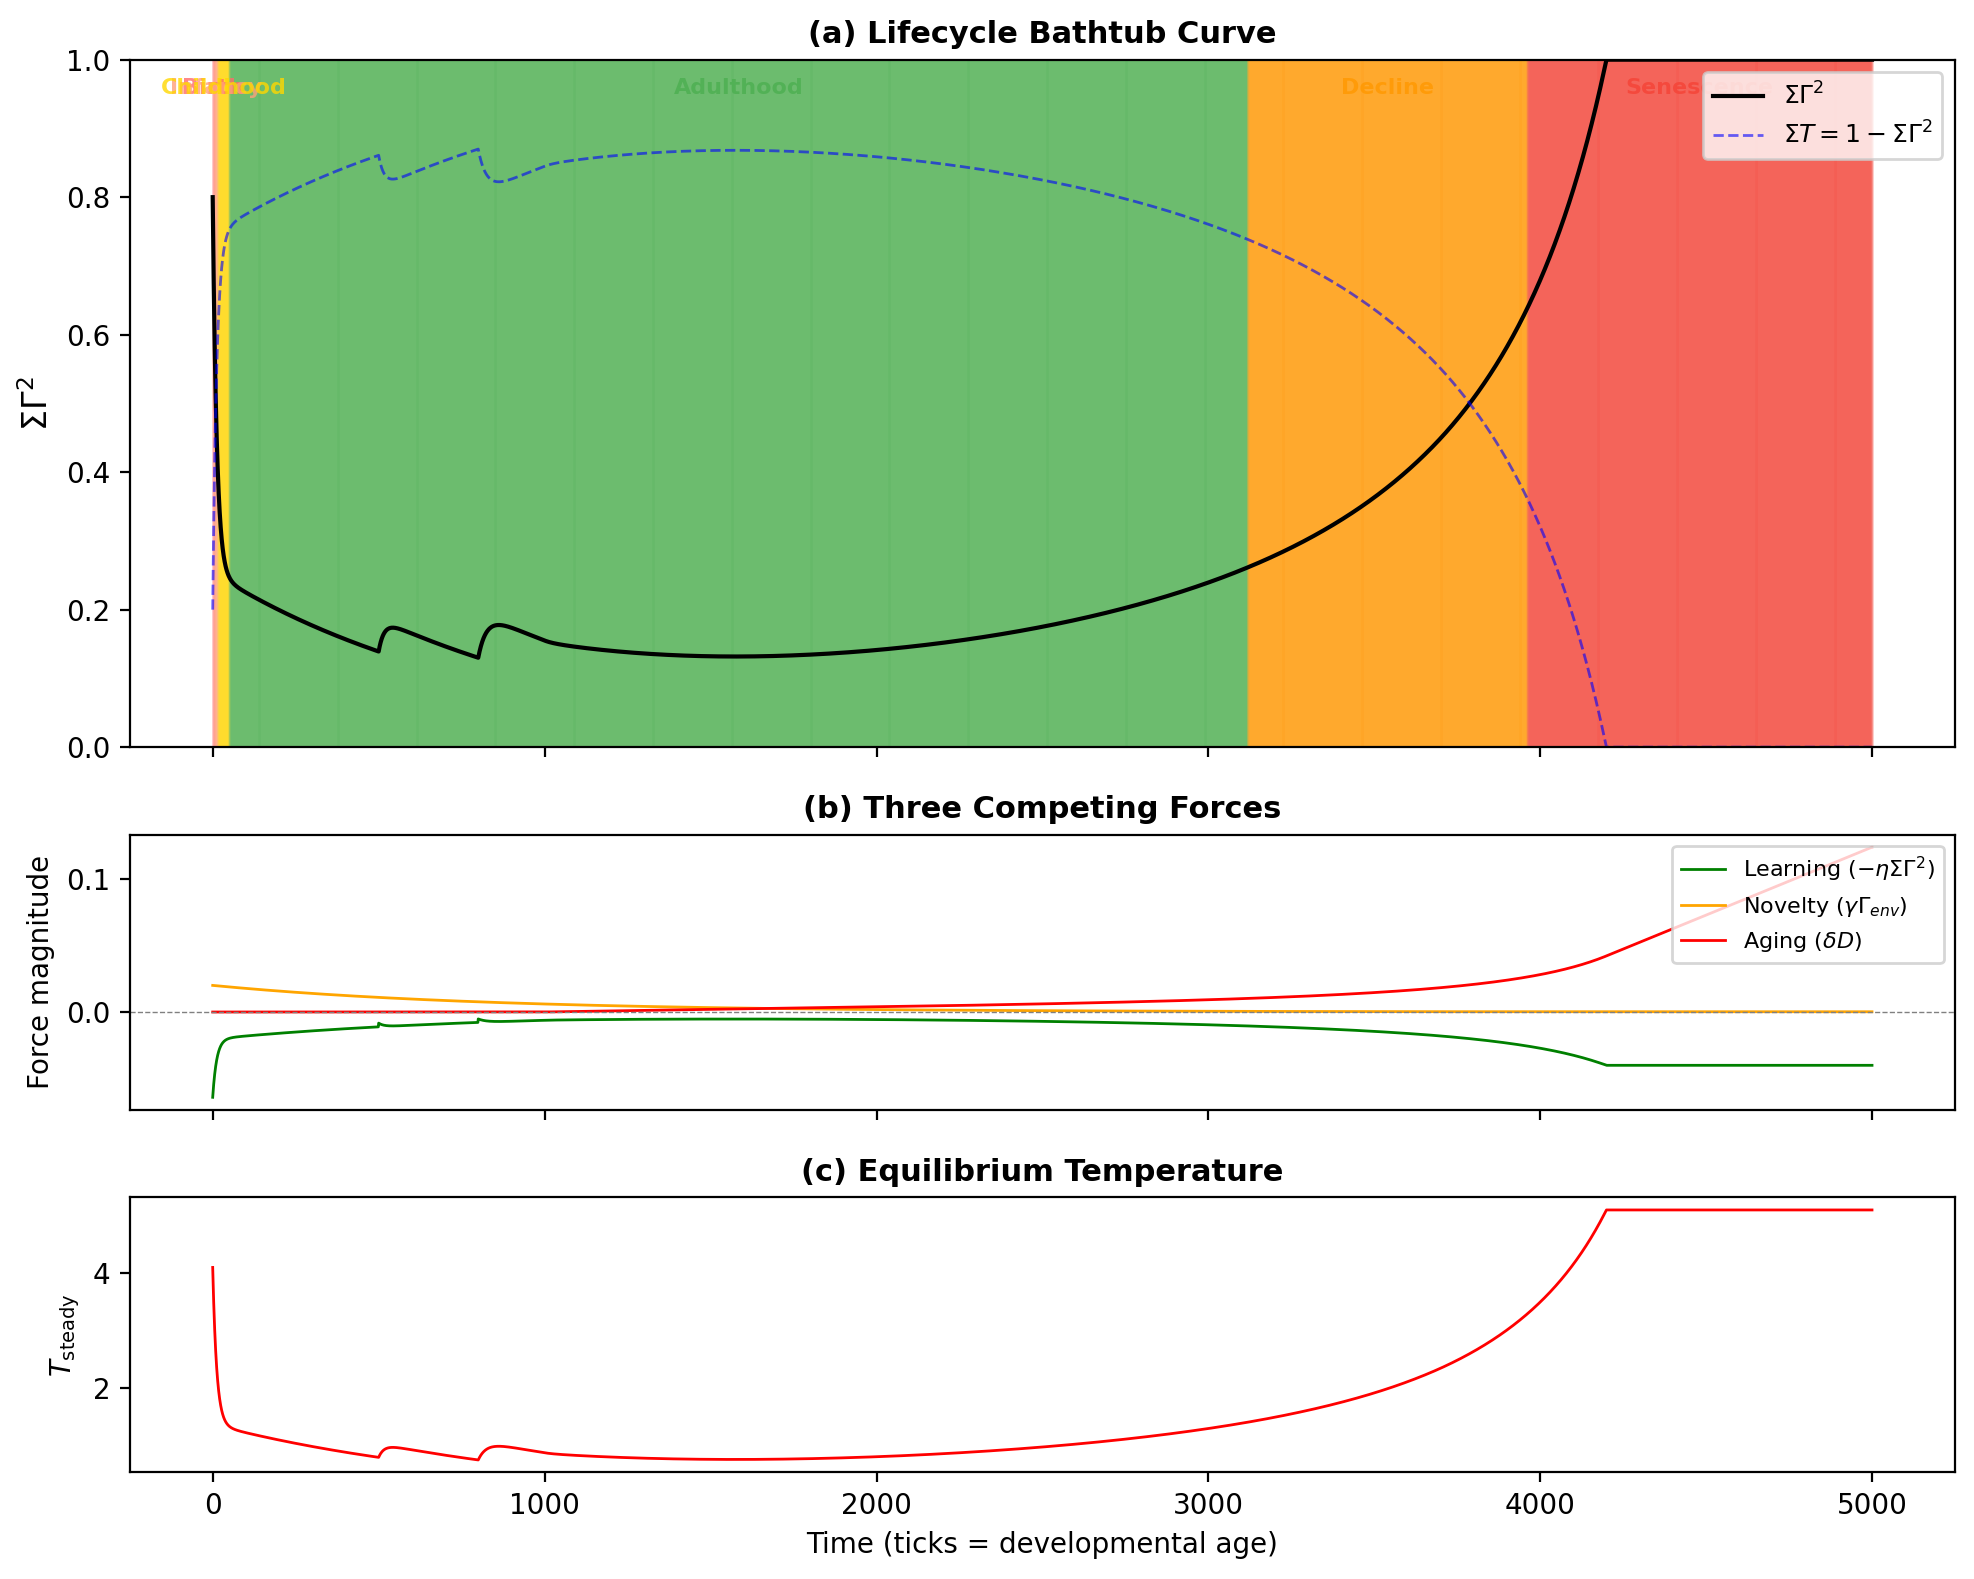
\includegraphics[width=\textwidth]{../figures/paper_iv_bathtub.png}
  \caption{Lifecycle bathtub curve (Experiment~1).
  (a)~$\Sigma\Gamma^2$ trajectory from birth to senescence;
  coloured bands indicate detected developmental phases.
  Blue dashed line: cognitive throughput $\Sigma T = 1 - \Sigma\Gamma^2$.
  (b)~The three competing forces: learning (green), novelty (orange),
  aging (red). The crossover points determine phase transitions.
  (c)~Equilibrium temperature $T_{\mathrm{steady}}$
  (Eq.~\eqref{eq:equilibrium}) tracks $\Sigma\Gamma^2$;
  it stabilises during adulthood.}
  \label{fig:bathtub}
\end{figure*}


\subsection{Experiment~2: Yerkes--Dodson inverted-U}
\label{sec:exp2}

Arousal is parameterised as a multiplier on both
$\eta$ and $\gamma$, with $\gamma$ scaling faster
than $\eta$ above moderate arousal.
We swept arousal from 0 to 1 at fixed
$\Gamma_{\mathrm{env}} = 0.5$ and measured
$\Sigma\Gamma^2$ after 100-tick learning blocks.

\emph{Verification criteria}:
(a)~performance---$(1 - \Sigma\Gamma^2)$---peaks at
intermediate arousal ($\sim$0.3--0.5);
(b)~performance degrades at both low and high arousal
(Fig.~\ref{fig:yerkes}, panel~a).

\begin{figure}[t]
  \centering
  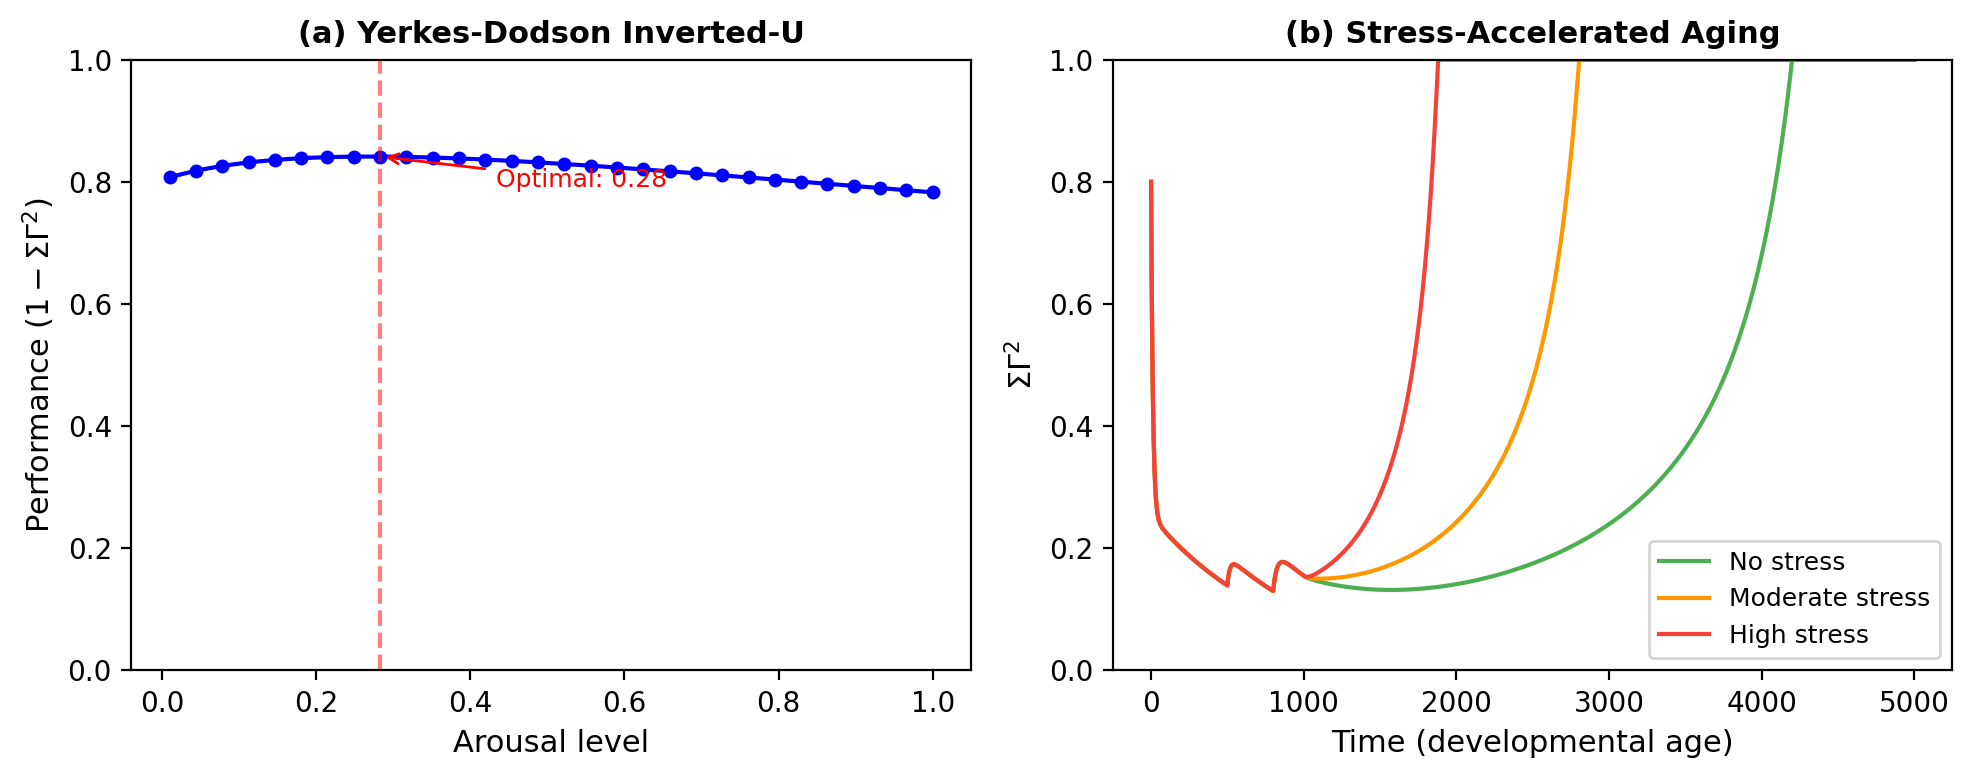
\includegraphics[width=\linewidth]{../figures/paper_iv_yerkes_stress.png}
  \caption{(a)~Yerkes--Dodson inverted-U: performance
  peaks at intermediate arousal where learning rate
  $\eta$ optimally exceeds novelty injection $\gamma$.
  (b)~Stress-accelerated aging: chronic stress
  (Arrhenius factor, Eq.~\eqref{eq:arrhenius-aging})
  causes earlier onset and steeper rise of the
  senescence phase.}
  \label{fig:yerkes}
\end{figure}


\subsection{Experiment~3: Repeated exposure adaptation}
\label{sec:exp3}

A fixed stimulus is presented 200 times.
We track $\Gamma$ at the stimulus-specific interface.

\emph{Verification criteria}:
(a)~$\Gamma$ drops monotonically from $\sim$0.7 to
$< 0.3$;
(b)~learning curve shows exponential decay
(fast early, slow late).


\subsection{Experiment~4: Chronic stress impairs learning}
\label{sec:exp4}

Two agents are simulated: one at $\sigma_{\mathrm{stress}}
= 0$ (relaxed), one at $\sigma_{\mathrm{stress}} = 0.7$
(chronically stressed).
Both receive identical stimuli for 500 ticks.

\emph{Verification criteria}:
(a)~stressed agent's $\Sigma\Gamma^2$ is higher than
relaxed agent throughout;
(b)~stressed agent's aging rate is $> 2\times$ baseline;
(c)~learning efficiency ($ -d\Gamma^2/dt$ per exposure)
is lower for the stressed agent.


\subsection{Experiment~5: Sleep--aging decomposition}
\label{sec:exp5}

An agent is run for 2000 ticks with periodic sleep
(every 96 wake ticks, 32 sleep ticks).
We measure (a)~daily $\Sigma\Gamma^2$ after sleep
(elastic recovery), and (b)~trend of daily minimum
$\Sigma\Gamma^2$ over time (plastic accumulation).

\emph{Verification criteria}:
(a)~sleep reduces $\Sigma\Gamma^2$ each night;
(b)~baseline $\Sigma\Gamma^2$ drifts upward over
many cycles (irreversible aging);
(c)~elastic/plastic ratio separated correctly.


\subsection{Experiment~6: Curiosity-driven exploration}
\label{sec:exp6}

An agent in a boring environment (constant stimulus,
$\Gamma_{\mathrm{env}} \to 0$) is given the option
to ``explore'' (receive novel stimulus at cost of
temporary $\Gamma^2$ increase).

\emph{Verification criteria}:
(a)~boredom accumulates when $|d\Gamma^2/dt| < \epsilon$;
(b)~spontaneous exploration triggers above boredom
threshold;
(c)~post-exploration $\Gamma^2$ is lower than
pre-exploration (net benefit).


\subsection{Experiment~7: Metacognition System 1/2 switching}
\label{sec:exp7}

Cognitive tasks of varying difficulty are presented.
We track $\Gamma_{\mathrm{think}}$ and observe
System~1/2 transitions.

\emph{Verification criteria}:
(a)~easy tasks ($\Gamma_{\mathrm{think}} < 0.3$):
System~1 (fast, automatic);
(b)~hard tasks ($\Gamma_{\mathrm{think}} > 0.6$):
System~2 (slow, deliberate);
(c)~hysteresis in switching (different engage/disengage
thresholds).


\subsection{Experiment~8: Novel stimulus shock and recovery}
\label{sec:exp8}

A well-adapted agent (low $\Sigma\Gamma^2$) is suddenly
exposed to a drastically novel environment.

\emph{Verification criteria}:
(a)~$\Sigma\Gamma^2$ spikes acutely;
(b)~recovery follows exponential decay;
(c)~post-recovery $\Sigma\Gamma^2$ is slightly lower
than pre-shock (net learning from the experience).


\subsection{Experiment~9: Full lifecycle simulation}
\label{sec:exp9}

The complete lifecycle is simulated with all three
forces active, sleep cycles, stress episodes, and
environmental novelty variation.

\emph{Verification criteria}:
(a)~six developmental phases emerge in correct order;
(b)~$\Sigma\Gamma^2$ trajectory matches bathtub curve;
(c)~$\Sigma T$ (cognitive throughput) peaks in adulthood;
(d)~Equilibrium temperature $T_{\mathrm{steady}}$
stabilises during adult phase.

\begin{figure}[t]
  \centering
  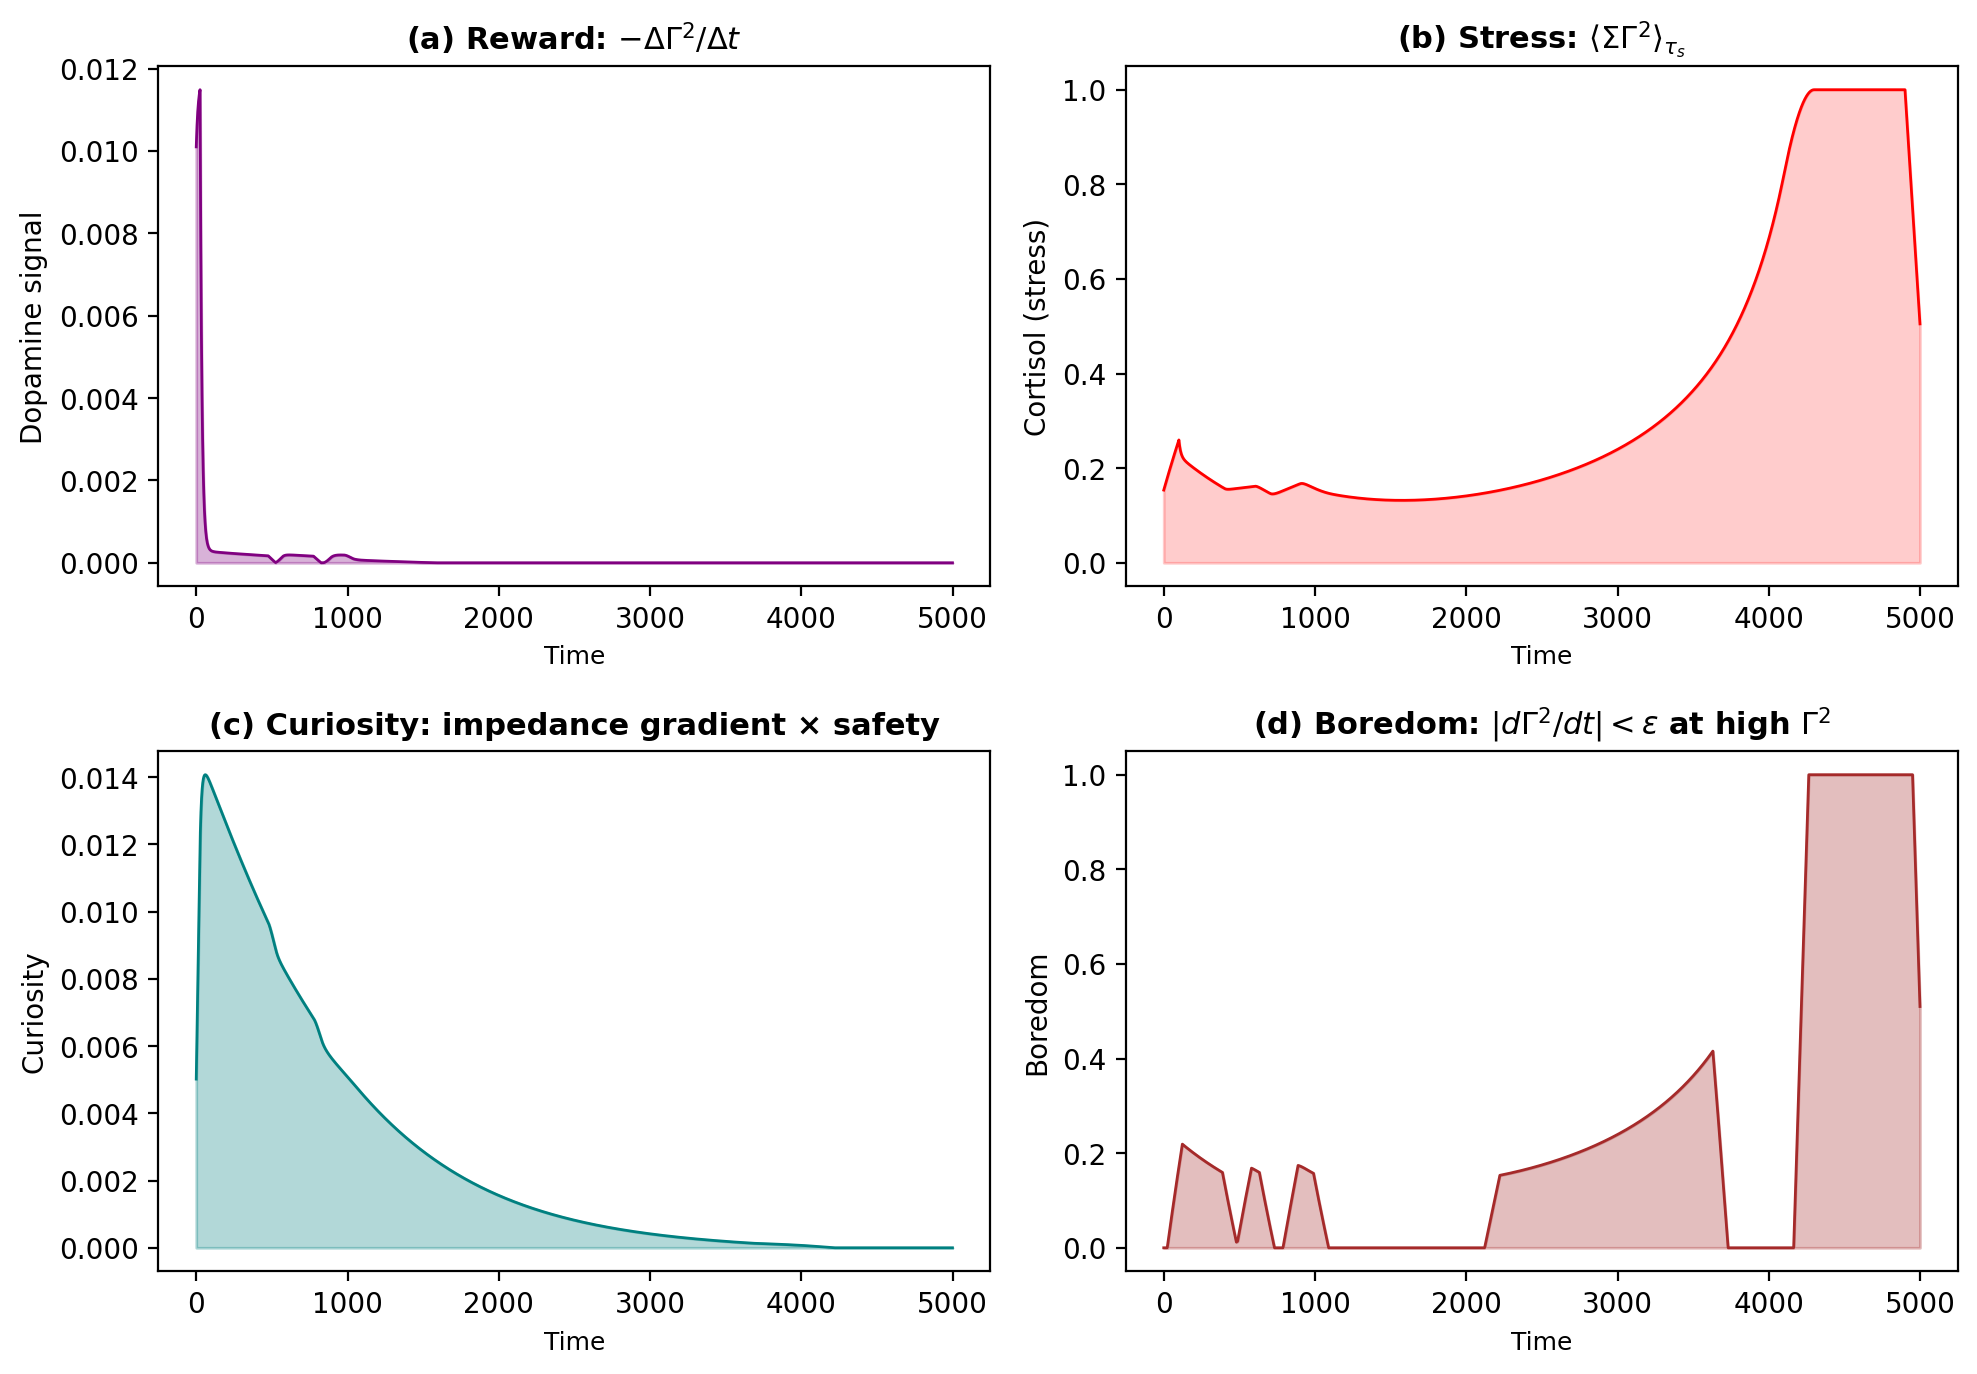
\includegraphics[width=\linewidth]{../figures/paper_iv_emotions.png}
  \caption{Emotion as $\Gamma^2$-dynamics readout (Experiments~6--9).
  (a)~Dopamine ($-\Delta\Gamma^2/\Delta t$): peaks during rapid
  learning in infancy/childhood, diminishes in stable adulthood.
  (b)~Cortisol (slow-averaged $\Sigma\Gamma^2$): highest at birth,
  lowest in adulthood, rising again in senescence.
  (c)~Curiosity (impedance gradient $\times$ safety): strongest
  in early development when gradients are steep.
  (d)~Boredom ($|d\Gamma^2/dt| < \epsilon$ at elevated $\Gamma^2$):
  emerges in late adulthood and decline phases.}
  \label{fig:emotions}
\end{figure}


% ============================================================
%  SECTION 8 — DISCUSSION
% ============================================================
\section{Discussion}
\label{sec:discussion}

\subsection{Methodological caveat: internal vs.\ empirical validation}

All nine computational experiments in this paper use the
Alice $\Gamma$-Net simulator, whose modules are built from
the very axioms (C1--C3) being tested.
The bathtub curve, Yerkes--Dodson optimum, and Coffin--Manson
aging all emerge because the simulator \emph{encodes} the
Lifecycle Equation---not because it independently confirms it.
This is a consistency check, not an empirical test.
True validation requires longitudinal impedance measurements
across the human lifespan (e.g.\ EEG coherence from birth to
senescence), which no group has yet attempted within this
framework.

\subsection{Unification of developmental psychology}

The Lifecycle Equation reduces the entire
developmental trajectory---from neonatal chaos
through childhood rapid learning, adult stability,
and senescent decline---to three physical forces
acting on a single state variable $\Sigma\Gamma^2$.
Classic developmental theories---Piaget's stages~\cite{Piaget1952},
Vygotsky's zone of proximal development~\cite{Vygotsky1978},
and the critical-period hypothesis~\cite{Hensch2005}---
emerge as parameter regimes of the same ODE,
not as competing theories.

Piaget's stages correspond to the phase transitions
of Sec.~\ref{sec:bathtub} (the
$\Sigma\Gamma^2$ level at which qualitatively
different cognitive operations become possible).
Vygotsky's ZPD is the range of $\Gamma_{\mathrm{env}}$
for which the learning term can reduce $\Sigma\Gamma^2$
in a single session---stimuli too easy
($\Gamma_{\mathrm{env}} \ll \Sigma\Gamma^2$) produce
no gradient, stimuli too hard
($\Gamma_{\mathrm{env}} \gg \eta/\gamma$) overwhelm
the learning term.
Critical periods are intervals of enhanced $\eta(t)$
where rapid impedance matching is biologically
privileged.

Notably, the dual-network organ model of Paper~II~\cite{PaperII}
requires an analogous self-repair mechanism:
a linearised Hebbian term
$\Gamma_n(t+1) = \Gamma_n(t)(1-\eta_n)$ with $\eta_n = 0.008$
prevents neural impedance saturation and guarantees
global attractor stability across all 10~organ territories
(Paper~II, Table~IV).
This mirrors the developmental learning term in~\eqref{eq:lifecycle}
and suggests a universal role for small, persistent
Hebbian corrections throughout the lifespan.

\subsection{Emotion as physics, not computation}

The reduction of emotion to impedance-mismatch dynamics
(Sec.~\ref{sec:emotion}) is not an analogy.
In the Alice Gamma-Net system, dopamine, cortisol,
curiosity, and boredom are \emph{computed} from
$\Gamma^2$ time series using the formulas
of Sec.~\ref{sec:emotion-detail}, and the resulting
behaviours---reward-seeking, stress avoidance,
exploration, and spontaneous action---emerge
without any additional ``emotion module.''
The distinction between cognitive and emotional
processing, which has troubled philosophy of mind
for centuries~\cite{Damasio1994}, dissolves:
both are readouts of the same impedance dynamics,
differing only in time scale and derivative order.


\subsection{Clinical implications}

The three-force framework generates clinical predictions:

(i)~\emph{Depression} as chronic high $\Sigma\Gamma_n^2$
with low $|d\Gamma_n^2/dt|$:
the neural network is mismatched but unable to learn
(boredom dynamics at system scale).
Treatment should increase $\eta_n$ (learning rate)
or decrease $\Gamma_{\mathrm{env}}$
(reduce environmental complexity).

(ii)~\emph{PTSD} as acute $\Gamma_n^2$ spike with
failure to decay:
the novelty term introduced a massive mismatch that
the learning term cannot resolve in normal time.
Treatment should provide controlled re-exposure
(titrated $\Gamma_{\mathrm{env}}$) to enable
gradual matching.

(iii)~\emph{ADHD} as excess novelty sensitivity:
$\gamma$ is chronically elevated, requiring
higher $\eta$ (stimulant medication increases
effective learning rate) to maintain
$d\Gamma^2/dt < 0$.

(iv)~\emph{Dementia} as accelerated neural aging:
$\delta_n \cdot D_n(t)$ overwhelms the learning term
at an earlier age than normal, producing premature
senescence---often preceded by vascular aging via
the cascade of Sec.~\ref{sec:aging-cascade}.

(v)~\emph{Hypertension} as chronic vascular mismatch:
$\Sigma\Gamma_v^2$ is elevated (undischarged vascular
impedance debt $D_{Z,v}$ from Paper~III~\cite{PaperIII}),
with vessel-wall $Z_v$ drifting above Murray's-Law optimum
(Paper~II~\cite{PaperII}).
Antihypertensive therapy reduces $\Gamma_v$ and preserves
material supply $\rho$, slowing downstream neural aging.

(vi)~\emph{Metabolic syndrome} as dual-network failure:
both $\Sigma\Gamma_n^2$ (cognitive decline, insulin resistance)
and $\Sigma\Gamma_v^2$ (hypertension, dyslipidemia) are
elevated simultaneously, placing the patient in the
``dual failure'' quadrant of Paper~II
($\Gamma_n^2 > 0.3$ and $\Gamma_v^2 > 0.3$,
$H \to 0$).


\subsection{Connection to Papers~I--III}

Paper~I established the \emph{spatial} structure
of impedance networks (relay nodes, fractal topology,
dimensional cut cost).
Paper~II established the \emph{vascular} extension
(Murray's Law, dual-network organ health
$H = (1-\Gamma_n^2)(1-\Gamma_v^2)$,
positive-feedback cascade).
Paper~III established the \emph{temporal} dynamics
(impedance debt $D_Z = D_{Z,n} + D_{Z,v}$,
sleep as dual-network debt discharge,
brain evolution, morphogenesis).
Paper~IV completes the series by establishing
the \emph{lifecycle} dynamics---how the dual-network
physics governs the complete arc from birth to death.

The four papers together provide a closed description:
the static architecture (Paper~I) determines the
channel structure $\{Z_i\}$;
the vascular extension (Paper~II) establishes the
dual-network organ model and the material-supply
coupling $I_{\mathrm{blood}} = (1-\Gamma_v^2)\,Q_0$;
the daily dynamics (Paper~III) determine the
sleep--wake cycle and its dual-network debt partition;
and the lifecycle dynamics (Paper~IV) determine the
developmental trajectory of \emph{both} networks.
The vascular--neural aging cascade
(Sec.~\ref{sec:aging-cascade}) is the lifecycle
manifestation of Paper~II's positive-feedback loop,
operating not on the tick-by-tick time scale of acute
disease but on the decade-long time scale of aging.
All four layers derive from a single variational
principle: Minimum Reflection Action,
$\mathcal{A}[\Gamma] = \int \Sigma|\Gamma|^2\,dt
\to \min$.


\subsection{Infant soft tissue as mechanical impedance buffer}
\label{sec:infant-buffer}

The neonatal body is characterised by soft cartilaginous
bones, thick subcutaneous fat, and highly elastic skin.
From an impedance standpoint, these tissues constitute
\emph{mechanical quarter-wave transformers} that provide
a graded impedance transition between the external
environment and the immature neural network:
\begin{equation}
  Z_{\text{infant}} \ll Z_{\text{adult}}\,,
  \qquad
  \Gamma_{\text{impact}} =
    \frac{Z_{\text{ground}} - Z_{\text{infant}}}
         {Z_{\text{ground}} + Z_{\text{infant}}}\,.
  \label{eq:infant-buffer}
\end{equation}
Because $Z_{\text{infant}}$ is low and graded (fat $\to$
cartilage $\to$ soft bone), the mechanical impact signal
is significantly attenuated before reaching nociceptors.
The same fall that would produce $|\Gamma|\approx 0.9$
in an adult skeleton produces
$|\Gamma|\approx 0.3$--$0.5$ in an infant.

This buffering is not incidental; it is a \emph{necessary}
design feature during the calibration phase ($t<t_1$).
With $\Sigma\Gamma^2\approx 0.8$ at birth
(Eq.~\ref{eq:novelty-term}), the neural network is
already saturated with mismatch from normal sensory input.
Injecting unattenuated mechanical pain signals would
overwhelm the calibration process, diverting the Hebbian
update (C2) toward pain-avoidance at the expense of
sensory-motor learning.

\subsection{Social referencing as external $\Gamma$ calibration}
\label{sec:social-gamma}

A well-documented developmental phenomenon is
\emph{social referencing}: when an infant falls, it
typically looks at the caregiver's face \emph{before}
deciding whether to cry~\cite{Sorce1985}.
If the caregiver displays alarm, the infant cries;
if the caregiver smiles, the infant resumes play.

Within the lifecycle framework, this behaviour is not
``learned'' but \emph{structurally necessary}.
The infant's pain-perception threshold is not yet
calibrated (the PFC decoder quality
$Q_{\text{PFC}}\ll 1$; Paper~V).
The caregiver's emotional expression provides an
external reflection coefficient $\Gamma_{\text{social}}$
that is superimposed on the mechanical signal:
\begin{equation}
  \Gamma_{\text{perceived}} =
    \Gamma_{\text{mechanical}} +
    \eta_{\text{social}}\,\Gamma_{\text{social}}\,,
  \label{eq:social-gamma}
\end{equation}
where $\eta_{\text{social}}\gg 1$ during infancy
(high social coupling) and
$\eta_{\text{social}}\to 0$ in adulthood
(self-calibrated system).

Each fall-and-look episode constitutes a Hebbian
calibration step for the pain threshold:
\begin{equation}
  \Delta Z_{\text{pain\_threshold}} =
    -\eta\,\Gamma_{\text{social}}\,
    x_{\text{pre}}\,x_{\text{post}}\,,
  \label{eq:social-hebbian}
\end{equation}
where $x_{\text{pre}}$ is the mechanical nociceptive
signal and $x_{\text{post}}$ is the behavioural response.
Over hundreds of such episodes, the infant's internal
pain threshold converges to a culturally and
environmentally appropriate set-point.

As myelination completes and $Q_{\text{PFC}}$ rises,
the system transitions from external calibration
($\eta_{\text{social}}\gg 1$) to autonomous operation
($\eta_{\text{social}}\to 0$).
This is the impedance-physics explanation for why
toddlers gradually stop looking at caregivers for
emotional cues after painful events.

\begin{remark}[Developmental design principle]
The infant body uses two complementary strategies---structural
buffering (soft tissue) and behavioural calibration (social
referencing)---to minimise $\Gamma^2$ during the
\emph{most vulnerable phase} of the lifecycle.
Both strategies are temporary scaffolding: bones harden
and social coupling decreases as the neural network
completes its self-calibration.
\end{remark}


% ============================================================
%  SECTION 9 --- CONCLUSION
% ============================================================
\section{Conclusion}
\label{sec:conclusion}

We have derived the Lifecycle Equation
(Eq.~\eqref{eq:lifecycle}):
a first-order ODE in which three forces---learning
(MRP descent), novelty injection, and Coffin--Manson
fatigue---compete to determine the complete cognitive
trajectory from birth to death.

The key results are:
\begin{enumerate}
  \item The bathtub curve of cognitive performance
    emerges from three physically motivated terms
    with no fitted function.
  \item Emotion (reward, pain, stress, curiosity, boredom)
    reduces to temporal readouts of $\Gamma^2$ dynamics
    at different time scales.
  \item The Yerkes--Dodson curve is the impedance-matching
    optimum between learning and novelty injection.
  \item Aging is Coffin--Manson fatigue accelerated
    by Arrhenius stress kinetics, with an irreversible
    (plastic) component that sleep cannot repair---operating
    in \emph{both} the neural and vascular networks.
  \item Atherosclerosis is vascular Coffin--Manson fatigue
    (Sec.~\ref{sec:vascular-aging}), and the vascular--neural
    aging cascade (Sec.~\ref{sec:aging-cascade}) explains
    why cardiovascular disease precedes and accelerates
    neurodegeneration.
  \item Death is positive-feedback collapse:
    $d^2(\Sigma\Gamma^2)/dt^2 > 0$ triggers
    runaway cascading failure, amplified by the
    dual-network cascade of Paper~II.
  \item Adulthood has a physical definition:
    the thermal steady state at which
    $d(\Sigma\Gamma^2)/dt = 0$.
\end{enumerate}

Together with Papers~I--III, the Lifecycle Equation
completes a four-layer description of biological
intelligence as Minimum Reflection Action on a
dual impedance network---from static architecture through
vascular topology and daily maintenance to the
complete arc of a life.


% ============================================================
%  ACKNOWLEDGMENTS
% ============================================================
\begin{acknowledgments}
The author thanks the open-source scientific Python community
and the developers of NumPy~\cite{Harris2020}.
\end{acknowledgments}


% ============================================================
%  DATA AND CODE AVAILABILITY
% ============================================================
\section*{Data and Code Availability}

All simulation code, including the
\texttt{LifecycleEquationEngine},
\texttt{PinchFatigueEngine},
\texttt{CuriosityDriveEngine},
\texttt{ImpedanceAdaptationEngine},
and \texttt{MetacognitionEngine}
modules, is available at
\url{https://github.com/cyhuang76/alice-gamma-net}
under AGPL-3.0.


% ============================================================
%  REFERENCES
% ============================================================
\begin{thebibliography}{99}

\bibitem{PaperI}
Hsi-Yu~Huang,
``Minimum reflection principle in heterogeneous impedance networks:
Irreducibility of dimensional cut cost,''
Zenodo (2026).
\href{https://doi.org/10.5281/zenodo.18847656}{doi:10.5281/zenodo.18847656}

\bibitem{PaperII}
Hsi-Yu~Huang,
``Twin impedance networks: A unified neural--vascular organ model
from the minimum reflection action,''
Zenodo (2026).

\bibitem{PaperIII}
Hsi-Yu~Huang,
``The cost of life: Impedance debt as the thermodynamic
origin of sleep and brain evolution,''
Zenodo (2026).
% DOI to be inserted upon publication

\bibitem{Kail1991}
R.~Kail,
``Developmental change in speed of processing during childhood
and adolescence,''
\emph{Psychol.\ Bull.}\ \textbf{109}, 490 (1991).

\bibitem{McEwen1998}
B.~S.~McEwen,
``Stress, adaptation, and disease: Allostasis and allostatic load,''
\emph{Ann.\ N.Y.\ Acad.\ Sci.}\ \textbf{840}, 33 (1998).

\bibitem{Salthouse2010}
T.~A.~Salthouse,
\emph{Major Issues in Cognitive Aging}
(Oxford University Press, 2010).

\bibitem{Coffin1954}
L.~F.~Coffin,
``A study of the effects of cyclic thermal stresses
on a ductile metal,''
\emph{Trans.\ ASME}\ \textbf{76}, 931 (1954).

\bibitem{Huttenlocher1979}
P.~R.~Huttenlocher,
``Synaptic density in human frontal cortex---developmental
changes and effects of aging,''
\emph{Brain Res.}\ \textbf{163}, 195 (1979).

\bibitem{Klutke2003}
G.~A.~Klutke, P.~C.~Kiessler, and M.~A.~Wortman,
``A critical look at the bathtub curve,''
\emph{IEEE Trans.\ Reliab.}\ \textbf{52}, 125 (2003).

\bibitem{Schultz1997}
W.~Schultz, P.~Dayan, and P.~R.~Montague,
``A neural substrate of prediction and reward,''
\emph{Science}\ \textbf{275}, 1593 (1997).

\bibitem{YerkesDodson1908}
R.~M.~Yerkes and J.~D.~Dodson,
``The relation of strength of stimulus to rapidity
of habit-formation,''
\emph{J.\ Comp.\ Neurol.\ Psychol.}\ \textbf{18}, 459 (1908).

\bibitem{Kahneman2011}
D.~Kahneman,
\emph{Thinking, Fast and Slow}
(Farrar, Straus and Giroux, 2011).

\bibitem{Alter2009}
A.~L.~Alter and D.~M.~Oppenheimer,
``Uniting the tribes of fluency to form a metacognitive nation,''
\emph{Pers.\ Soc.\ Psychol.\ Rev.}\ \textbf{13}, 219 (2009).

\bibitem{Walker2017}
M.~P.~Walker,
\emph{Why We Sleep: Unlocking the Power of Sleep and Dreams}
(Scribner, 2017).

\bibitem{Ohayon2004}
M.~M.~Ohayon, M.~A.~Carskadon, C.~Guilleminault,
and M.~V.~Vitiello,
``Meta-analysis of quantitative sleep parameters from
childhood to old age in healthy individuals,''
\emph{Sleep}\ \textbf{27}, 1255 (2004).

\bibitem{Mander2017}
B.~A.~Mander, J.~R.~Winer, and M.~P.~Walker,
``Sleep and human aging,''
\emph{Neuron}\ \textbf{94}, 19 (2017).

\bibitem{Epel2004}
E.~S.~Epel \emph{et al.},
``Accelerated telomere shortening in response to life stress,''
\emph{Proc.\ Natl.\ Acad.\ Sci.\ U.S.A.}\ \textbf{101},
17312 (2004).

\bibitem{sprint2019}
SPRINT MIND Investigators,
``Effect of intensive vs standard blood pressure control on
probable dementia: A randomized clinical trial,''
\emph{JAMA}\ \textbf{321}, 553 (2019).

\bibitem{Lupien2009}
S.~J.~Lupien, B.~S.~McEwen, M.~R.~Gunnar, and C.~Heim,
``Effects of stress throughout the lifespan on the brain,
behaviour and cognition,''
\emph{Nat.\ Rev.\ Neurosci.}\ \textbf{10}, 434 (2009).

\bibitem{Piaget1952}
J.~Piaget,
\emph{The Origins of Intelligence in Children}
(International Universities Press, 1952).

\bibitem{Vygotsky1978}
L.~S.~Vygotsky,
\emph{Mind in Society: The Development of Higher
Psychological Processes}
(Harvard University Press, 1978).

\bibitem{Hensch2005}
T.~K.~Hensch,
``Critical period plasticity in local cortical circuits,''
\emph{Nat.\ Rev.\ Neurosci.}\ \textbf{6}, 877 (2005).

\bibitem{Damasio1994}
A.~R.~Damasio,
\emph{Descartes' Error: Emotion, Reason, and the Human Brain}
(Avon Books, 1994).

\bibitem{Harris2020}
C.~R.~Harris \emph{et al.},
``Array programming with NumPy,''
\emph{Nature}\ \textbf{585}, 357 (2020).

\bibitem{Sorce1985}
J.~F.~Sorce, R.~N.~Emde, J.~J.~Campos, and
M.~D.~Klinnert,
``Maternal emotional signaling: its effect on the
visual cliff behavior of 1-year-olds,''
\emph{Dev.\ Psychol.}\ \textbf{21}, 195 (1985).

\end{thebibliography}

\end{document}
